\chapter{Introduction}

Hydrogen Bonding (HB) is one of the most important non-covalent chemical
interactions, in this thesis we will work around that interaction, through the
use of Quantum Chemistry tools such as Electron Localization Function (ELF) and
Interacting Quantum Atoms (IQA) our systems have been analysed, and as shown
in \citet{Munrriz2019}, with those tools simple correlations have been found,
and can be explained with elementary models such as the homogeneous electron
gas.

Published papers as \citet{Toche2016} and \citet{Castor2020} have analysed
topology in water cluster, where the IQA partition was done through electron
density analysis by Quantum Theory of Atoms In Molecules. In this thesis we
will approach the IQA partition using the ELF, with the help of
{\sc{Promelf}}~\cite{promolden} code.

To approach the problem of HB in water clusters, we studied different
clusters not only modifying the size of the clusters, but also with multiple
arrangements for the same cluster size. The clusters were treated by
DFT calculations to obtain the energy and wavefunction, with these
results we made the ELF analysis, which allows us to compute
the IQA electronic energy partition.

%Our results show that the exchange-correlation contribution is one of the most
%important contributions not only for the HB interaction, even for the whole system,
%\textit{i. e.}, the HB helps to minimize the electronic energy in water
%clusters.
%
%Moreover, many contributions to the HB interactions are related with the
%population of the lone electron pair basins but not for the H basins.
%In
%contrast, the sum over all contributions for potential, kinetic and
%exchange-correlation energies are correlated for lone electron pairs and H
%basins.

\newpage
%\pagebreak
%
\section{Water}

In ancient times water was considered as an element, it was not until 1781
Henry Cavendish (1731-1810) postulated that water is a combination of simpler
elements and the first proof provided that water is made by two volumes of H
for every volume of O was developed by Gay-Lussac in 1804~\cite{sanchez2006revolucion}.
Nowadays it is well known that the water molecule is composed of two hydrogen
atoms interacting by a single bond with a central oxygen atom that has two lone
electron-pairs.

The lone electron-pairs are know to play an indispensable role in describing
not only structures but also reactivity of molecules. Classically, a lone pair
is defined as a valence electron pair, bound to a nucleus, not utilized in
chemical bonding~\cite{Lee1996-hp}. However, author as \citet{Kumar2014}
brought together various quantum mechanical perspectives to describe the lone
electron-pairs, along Bonding Theories, Molecular Electrostatic Potential, and
Scalar Fields as QTAIM. And as we will discuss in Section \ref{elftheory} they
are also related with the ELF.

Work as the published by \citet{Gallivan1999} even approach if the electron
pairs in water can have a binding interaction with a $\pi$ system such as the
$\pi$ that lies in hexafluorobenzene, concluding with an affirmative answer to
the presence of an attractive interaction. Remarking the importance of
those lone electron-pairs.

The electron pairs mentioned above confer particular properties to
water~\cite{biology}. Some of those properties are:
$i$) water has an autoprotolysis equilibrium~\cite{mcmurry},
$ii$) the ionic mobility of the hydronium ion in water is high due to the migration mechanism~\cite{voet},
$iii$) water has a high surface tension value (\SI{72.88}{\milli \newton \per \meter} at \SI{20}{\celsius}) due to the strong cohesion of its molecules~\cite{dean92:LHC},
$iv$) water has high melting and boiling points, compared to other hydrogen chalcogenides~\cite{morrison},
$v$) water has a negative melting volume change, so the density of the liquid state is greater than that of the solid state~\cite{serway2001fisica},
$vi$) the value of the fusion enthalpy of water is unusually large,
\SI{333.6}{\joule \per \gram} a \SI{0}{\celsius}~\cite{noauthororeditor2007handbook}.
The above properties, among many others, make water a molecule worthy of several theoretical and experimental studies.


%\subsubsection{Proton desintegration}

%One the one hand, in hte Standar Model of Particle Physics, the protons are
%theoretically stable, that because the conservation of baryon
%number~\cite{standarmodel}. By the other hand, are some hypothesis in some
%field theories that breaks explicitly the symmetry about the baryon number,
%allowing protons to decay into lighter charged particles..~\cite{Kuhne:2011zz}

%An experiment looking for the proton decay by Cherenkov radiation,
%that radiation should be produced by the decay
%of any proton in its ultra \SI{50}{\kilo\tonne} pure water, where the radiation
%should be measure by its \num{13} thousand photomultiplier tubes~\cite{Kamioka}.
%Fortunatly for chemistry or unfortunatly for physics, until now we do not have
%any experimental data about it. However, Super-Kamiokande observatory already
%gave important contributions, as for example, the strong evidence about
%neutrino oscillation, consistent with theories that neutrinos have
%a nozero-mass~\cite{10.2307/26058368}. With that Takaaki Kajita 
%and Arthur B. McDonald won the Physics Nobel Prize.

\newpage

\section{Hydrogen Bond}

\begin{wrapfigure}[13]{r}{0.41\textwidth} %this figure will be at the right
%\begin{figure}%{0.41\textwidth}
    \centering
    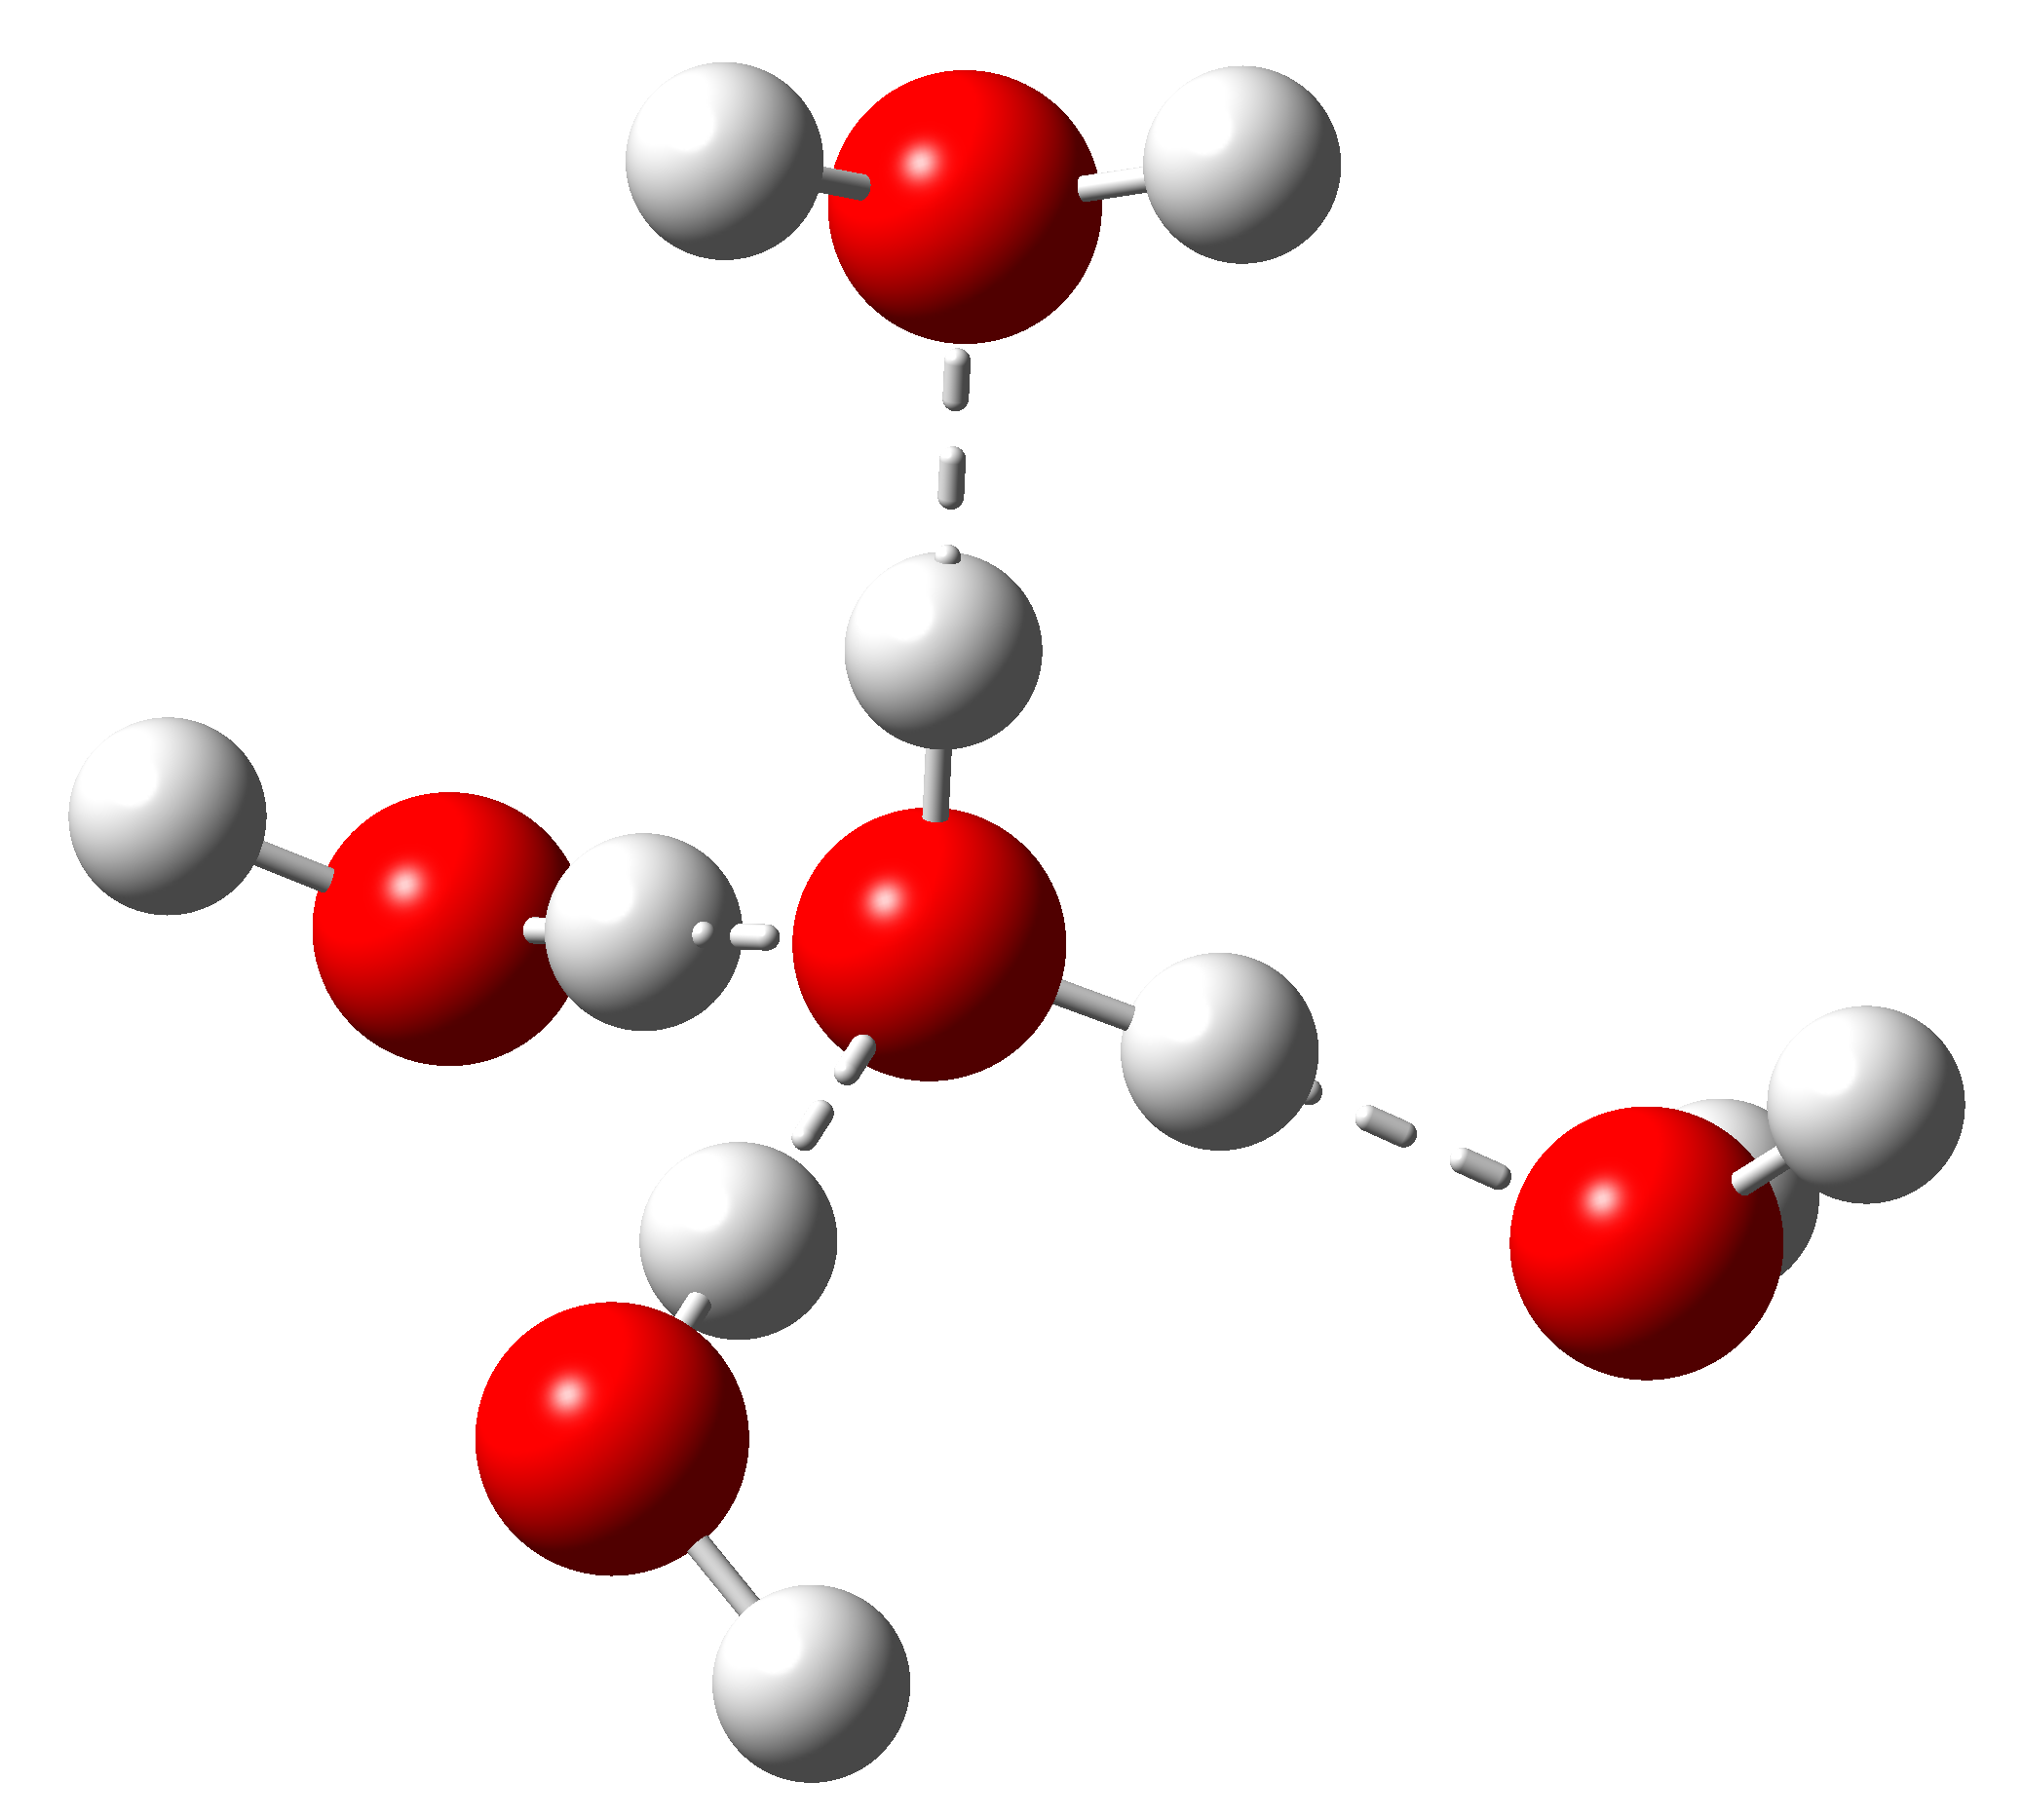
\includegraphics[width=0.41\textwidth]{2/img/4h2o}
    \caption{The central water molecule is accepting two hydrogen
    bonds and giving other two,
    then it can be said that the molecule has 4 HB, two of these
    as an acceptor and two as donor.}
    \label{4_h2o}
%\end{figure}
\end{wrapfigure}

Several of the water particular properties are mostly explained by an special
non-covalent interaction, the Hydrogen Bond (HB). The Figure \ref{4_h2o} shows
a cluster of five water molecules interacting by HBs. The total number of HB
interactions for a cluster that is as large as Avogadro constant ($N_A$) is
$2N_A$. This HB lattice gives the system a cohesion that is unusual for
hydrogen chalcogenides~\cite{smith2005}.

%\vspace*{1.5cm}
The HB was discovered more than one hundred years ago and it is not possible to
attribute this finding to a single author. Moreover, there is no published
paper that can be consider as the beginning of the term. Scientific papers
about HB start to appear at the end of XIX century, in particular in English
and German literature. However, the HB relevance was not enough
recognized and almost completely ignored~\cite{steiner,quane1990reception}.

%\newpage
%\pagebreak

\color{blue}
\begin{quote}
\textit{... there are several interesting ideas in this paper, but there is one
you'll never get chemists to believe: the idea that a hydrogen atom can be
bonded to two other atoms at the same time...}
\begin{flushright}
%\citeauthor{hildebrand1958wendell}
\citet{hildebrand1958wendell}
\end{flushright}
\end{quote}
\color{black}

Later studies developed around 1920~\citep{steiner} tried to explain certain
phenomena already known (the vapor phase density of hydrogen
fluoride, anomalous freezing points or vapor density curves of various liquid
mixtures~\cite{quane1990reception}), but with a new perspective.  ``\textit{The
idea of a hydrogen kernel held between two atoms as a theory in regard to
certain organic compounds}''~\citep{Latimer1920}, ``\textit{it seems that the
hydrogen nuclei instead of forming duplets with electrons in the same atom,
form duplets in which the two electrons are in different
atoms}''~\citep{Langmuir1921}.

\newpage

At that time only two research groups (Thomas Lowry of Cambridge University and
Nevil Sidgwick at Oxford) and Huggins (in two papers~\citep{Huggins1922,
Huggins1922_2}) use the concept of Hydrogen Bond, despite not using the term,
in contrast they use terms as ``coordination of hydrogen''~\cite{Sidgwick1924}.
In those works the H atom is bonded to two atoms.

The first one who used the term Hydrogen Bond was
Pauling in 1931~\citep{gilli}.  At the end of 1930 the HB was explained in
terms of classic electrostatic phenomena, it was approached in those terms
since the examples found at that time were only weak interactions. Currently,
the cases where the HB has a higher interaction energy are known, where the
non-classic contribution cannot be neglected, besides the very weak ones that
are mostly van der Waals.

The Hydrogen Bond interaction is classified as medium range interaction
(typically from 5 to 30 \SI{}{\kilo \joule \per \mole}), in view of the fact
that: $i$) the phenomenon appears over larger distances than covalent bonds
and is weaker than covalent bonds, $ii$) the conventional HB are not enough
weak to be classified as a dispersion force~\cite{chang}.
%it is not weak enough to be classified
%as a dispersion force.~\cite{chang}

%The next HB definition was proposed by Steiner~\cite{steiner}:
Steiner~\cite{steiner} proposed the following definition for HB:

\begin{quote} 
An X-H$\cdots$A interaction is called a ``Hydrogen Bond'' if $i$) it
constitutes a local bond, and $ii$) X-H acts as proton donor to A.
\end{quote}

\noindent This way of describing the HB is flexible enough to include a wide
range of phenomena, in which a non-covalent interaction around an H atom is
involved. The Steiner definition is valid from the simplest HB cases in which
the donor X has just one H able to interact with an acceptor A which has only
an electron-pair free to make the bond~\cite{scheiner}; and also for more
complex interactions as the HBs involved at proteins folding.

The \gls{IUPAC} defines the HB as follows:

\begin{quote}
The hydrogen bond is an attractive interaction between a hydrogen atom from a
molecule or a molecular fragment X–H in which X is more electronegative than H,
and an atom or a group of atoms in the same or a different molecule, in which
there is evidence of bond formation~\cite{iupac}.
\end{quote}

This definition goes far beyond the traditional HB definition usually found in
common textbooks, in which ones where HBs are more closed to interactions of H
with F, N or O. The IUPAC also provides a list of criteria used to
characterize hydrogen bonds, the list of criteria is based in theoretical and
experimental knowledge and evidence. Some of those criteria are~\citep{iupac}:

\begin{enumerate}

\item The forces involved in the formation of a hydrogen bond include those of
an electrostatic origin, those arising from charge transfer between the donor
and acceptor leading to partial covalent bond formation between H and Y, and
those originating from dispersion.

\item The X–H $\cdots$ Y angle is usually
linear (180$^{\circ}$) and the closer the angle is to 180$^{\circ}$, the stronger
is the hydrogen bond and the shorter is the $\mathrm{H}\cdots \mathrm{Y}$ distance.

\item The Gibbs energy of formation for the hydrogen bond should be greater
than the thermal energy of the system for the hydrogen bond to be detected
experimentally.

\end{enumerate}
%\pagebreak
\newpage

\section{Cooperativity and Anticooperativity of HB}

\begin{figure}[h]
\centering
\begin{subfigure}[b]{0.43\linewidth}
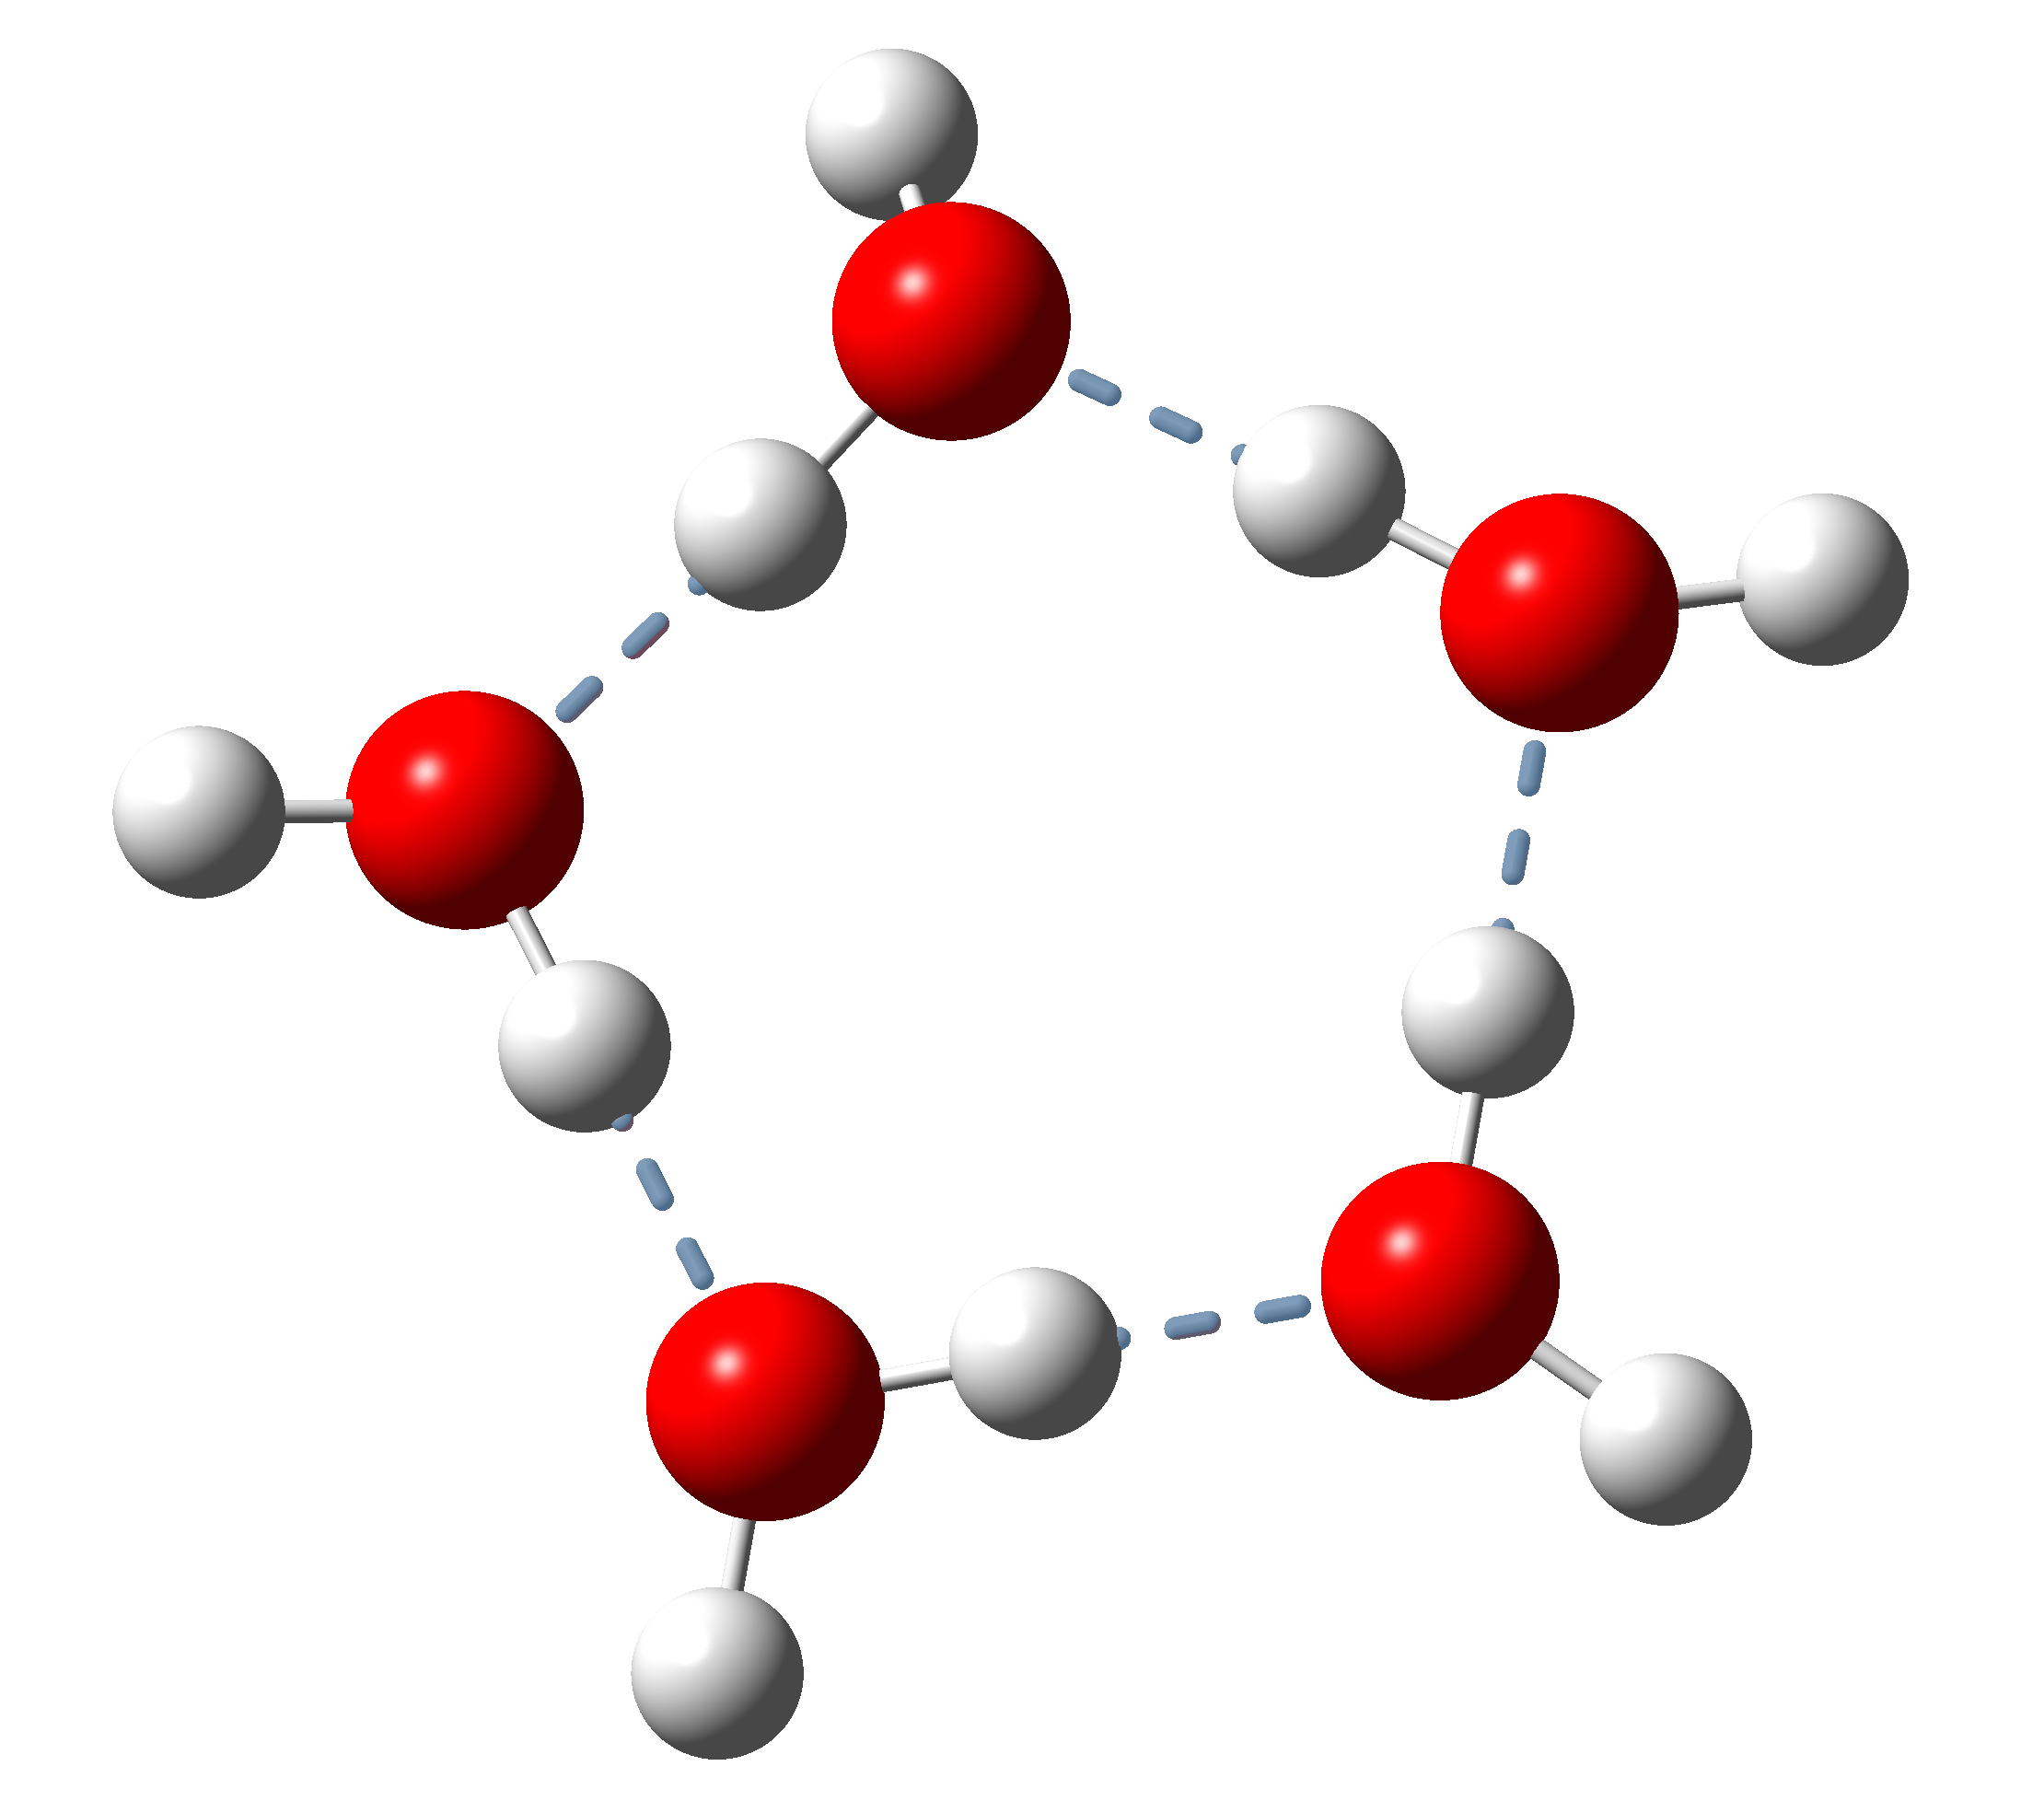
\includegraphics[width=\linewidth]{2/img/pentamero}
\caption{Homodromic case.}
\label{pentamero}
\end{subfigure}
\begin{subfigure}[b]{0.43\linewidth}
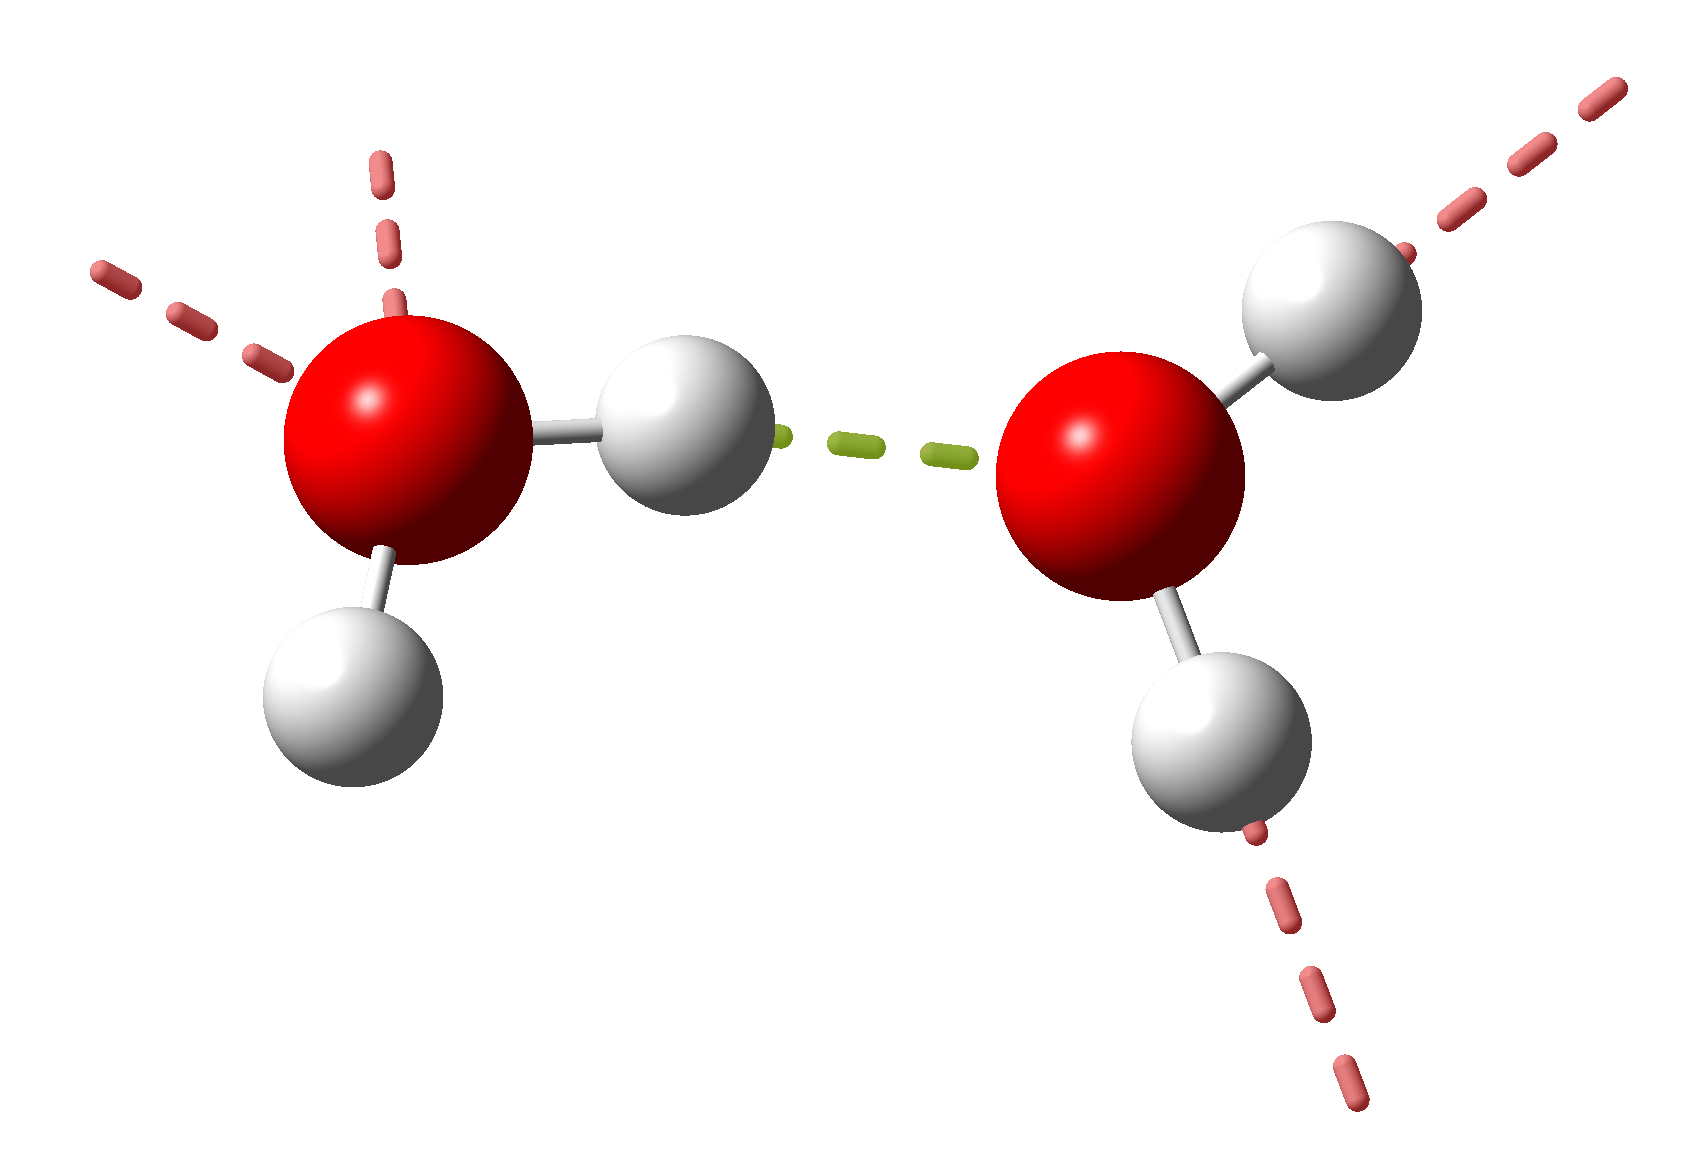
\includegraphics[width=\linewidth]{2/img/dimero_b}
\caption{Cooperative and anticooperative effects.}
%\label{dimero_b}
\label{coo_anti}
\end{subfigure}
%\begin{subfigure}[b]{0.3\linewidth}
%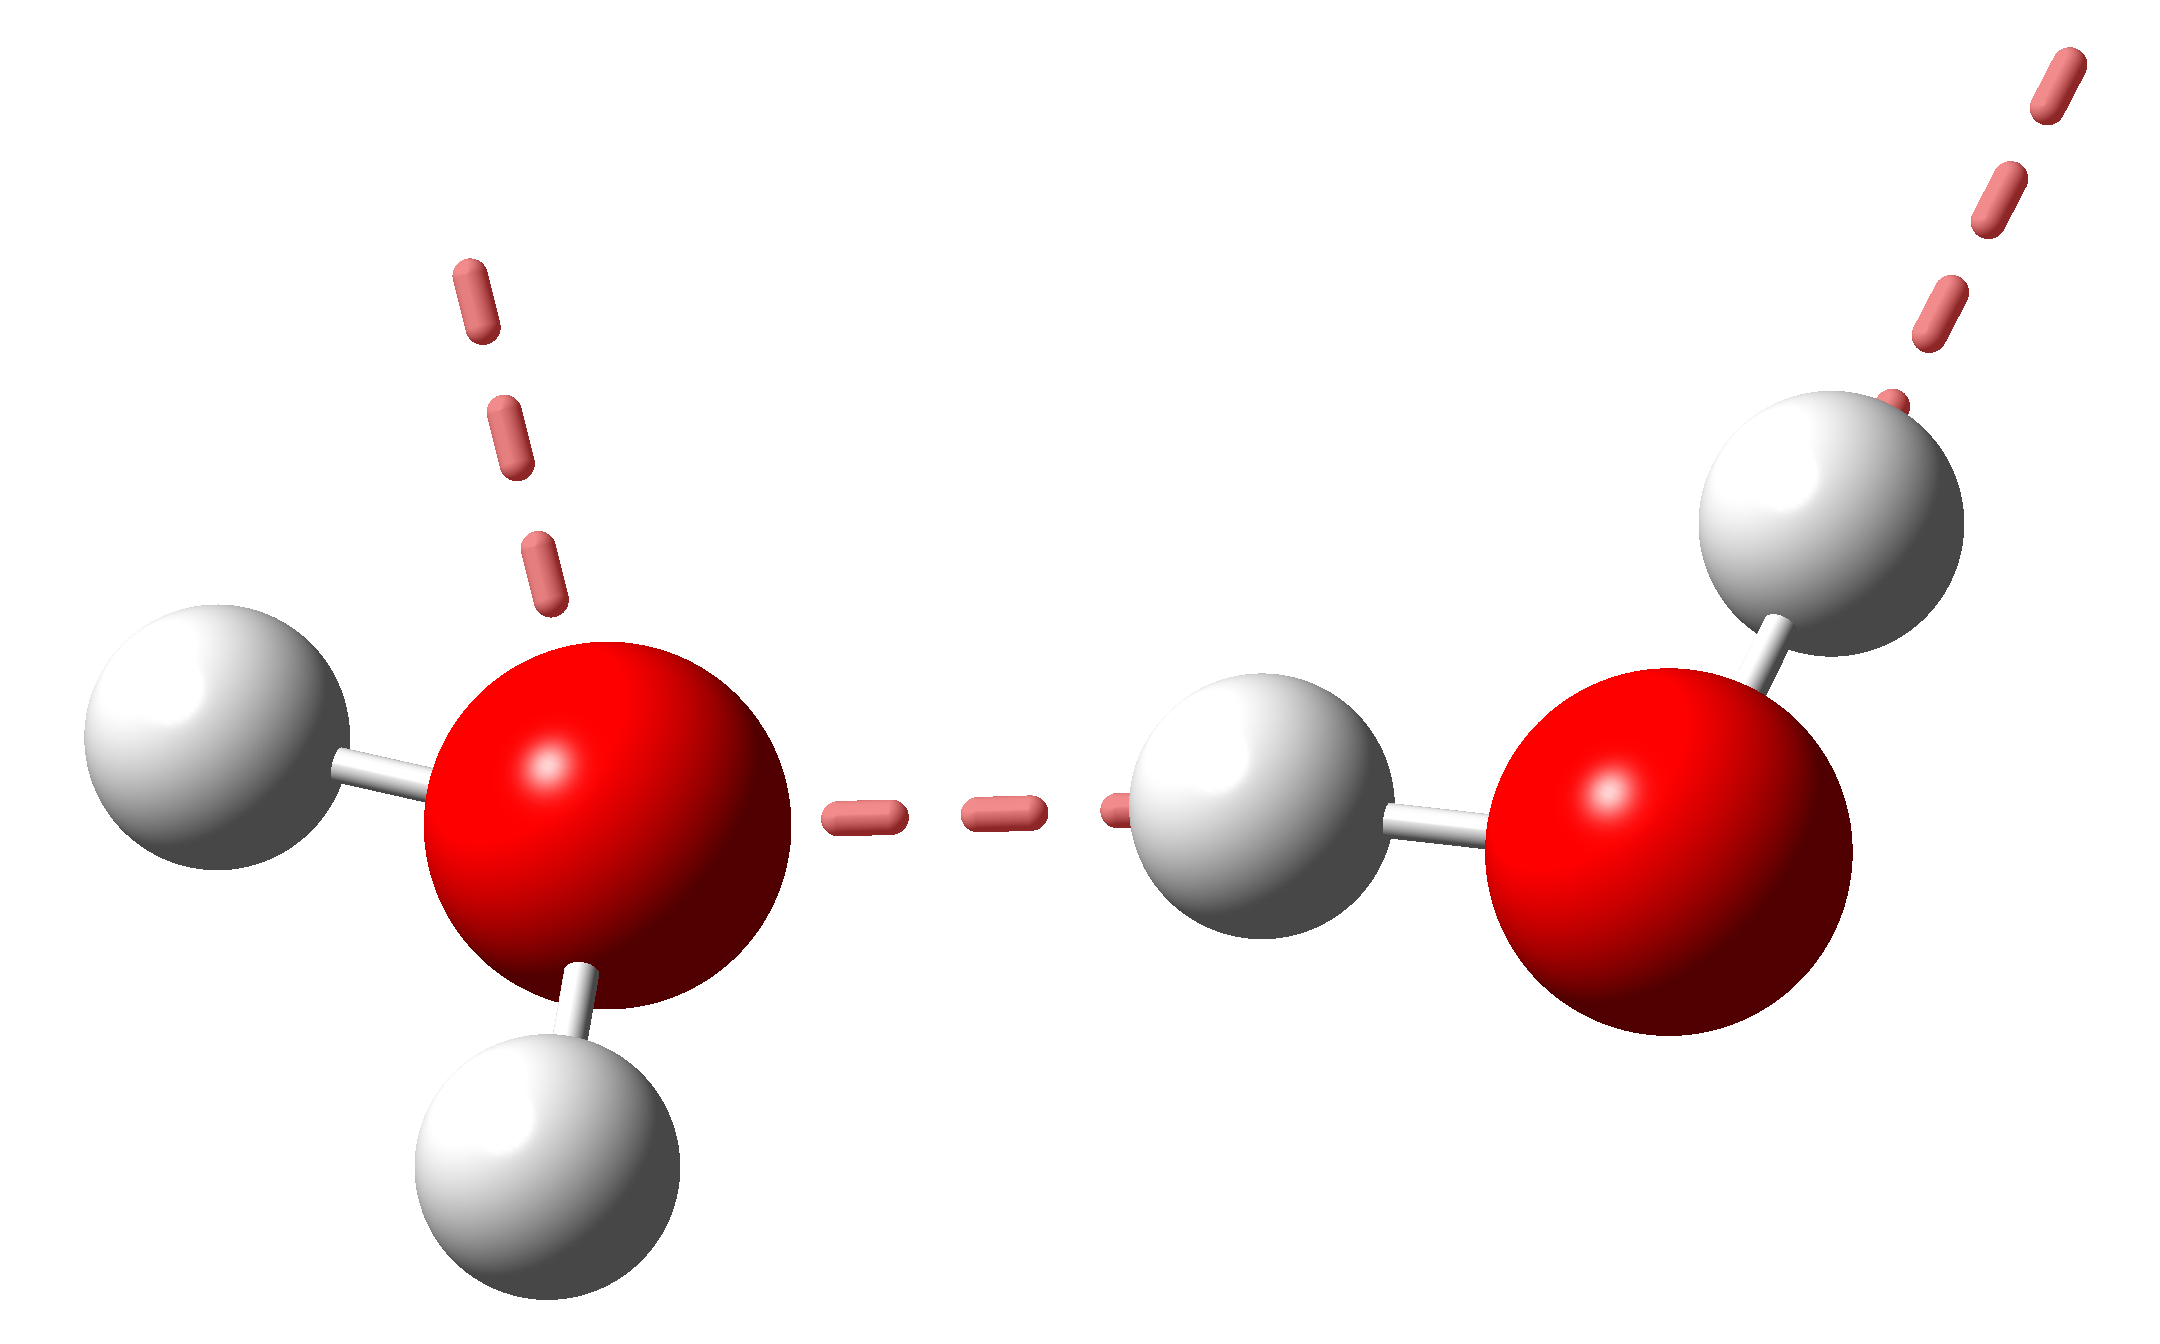
\includegraphics[width=\linewidth]{2/img/dimero_c}
%\caption{Anticooperative}
%\label{dimero_c}
%\end{subfigure}
\caption{Cooperative and anticooperative effects. In green the strongest HB (cooperative), in blue the homodromic interactions and
in red the weakest interactions (anticooperative).}
\label{fig_coop}
\end{figure}

The complexity of the HB lattice in water clusters comes from: $i$) the water
capacity to be donor and acceptor (even at the same time), $ii$)
%the variety of angles and directions of the HB.
the HBs encompass a broad distribution of forces and directions.
Then, in the three-dimensional real lattice there lie a
big variety of angles and distances for HB interactions~\cite{liu_science,
smith2005}. 

The cooperative and anticooperative effects found in water clusters
are one of the main phenomena characterizing HBs,
which can be found inside interaction lattices, as is
shown in Figure \ref{fig_coop}. 

Cooperative effects can be qualitatively rationalized in terms of
the acid-base behavior of each monomer, since the donor acid character
increases when the oxygen becomes protonated while its basic character increase
when the OH group gives its proton away~\cite{M1992}.

In Figure \ref{pentamero} a cyclic homodromic pentamer is shown \textit{i. e.,}
all the water molecules are accepting and giving a proton. 
While cooperative and anticooperative effects are shown in in Figure \ref{coo_anti},
for the cooperative case we need to note how $i$) the HB donor (left molecule) is
accepting two HBs, having a charge bereft, charge that can be recover by donating a HB, 
and $ii$) the HB acceptor (right molecule) is donating two HB,
being overcharged, charge that can be easily transferred by accepting a HB.

%Cooperative and
%anticooperative effects are shown in Figures \ref{dimero_b} and \ref{dimero_c},
%respectively. In the cooperative case \ref{dimero_b} is noted $i$) the donor
%molecule is accepting two H atoms, having a charge bereft, charge that can be
%recover by donating a HB, $ii$) the HB acceptor molecule is donating two HB,
%being overcharged, charge that can be easily transferred by accepting a HB.

In contrast, in the same system we will see also anticooperative effects, for
that we should thought the last two points trough the other four HB
interactions that the system has, where there are $i$) a HB donor that is
doubly charge deprived and $ii$) a HB acceptor being doubly overcharged.  These
effects at the same time results in an anticooperative phenomenon for the red
highlighted HB in Figure \ref{coo_anti}, not forgetting that the green one is
the interaction that exhibits the cooperative phenomenon. Therefore, in a same
system we can have both phenomena depending which HB is being analysed.

%In contrast, in the Figure \ref{dimero_c} it should be noted that $i$) the HB donor
%molecule is a double donor (right water molecule), having  more charge density
%than usual, and $ii$) the HB acceptor molecule (left water molecule) is
%accepting another H into a second HB, then it has a charge bereft. These
%effects at the same time results in an anticooperative phenomenon, since the
%two water molecules are in the least energetically favored situation for a
%HB interaction.
%two water molecules is in the least energetically favored for a HB interaction
%situation to lie in a HB interaction.

Work such as the ones carried out by \citet{M1992} show how Pople basis sets as
6-31G* overestimate the cooperative effects at HF level, whereas the
6-311+G(d,p) basis yields values closer to those obtained with much larger
basis.  As we will see in our work we also use a triple-$\zeta$ basis set but
Dunning instead of Pople, mainly because Dunning basis sets were developed for
post Hartree Fock methods~\cite{Dunning1989}.

The capability to act as a donor or acceptor in water molecules also depends on
the coordination of the molecule as shown in ~\citet{Toche2016, Castor2020}
where the tricoordinated (double donor, acceptor) water molecule is the best
acceptor and the tricoordinated (double acceptor, donor) is the best donor.
Particularly, those two cases are in our water clusters, thus, we intend to
forecast the same trend, a match between the ELF and electronic density topologies.

The above ideas are intended to be the cornerstone for this thesis, and through
a quick overview of the theory behind the quantum mechanical tools that we use,
we pretend to know how we will deal the problems that arise in
the realization of this thesis.

\chapter{Objectives}

Several researches of HB in water clusters have been proposed, one of those is
the description of the HB interactions between water molecules by the
\gls{ELF}.

The principal objective of this thesis is the study of HB interaction through
an IQA analysis of the ELF, with the particularity hypothesis that the ELF can give us
enough information necessary to understand the HB in water clusters. In particular,
to improve on previous knowledge published in the scientific literature on IQA partitioning of ELF and water clusters,
the next points are searched

\begin{enumerate}

\item Describe the HB by an ELF analysis and if possible in different ways.

\item Analyse the non-covalent interactions and how those interactions
are related with the ELF.

\item Analyse how the exchange-correlation and classical contributions are in
HB interactions.

\item A computational goal is to compute all systems with {\sc{Promelf}}
code~\cite{promolden},
since researchers how have already used the code have had problems with
``big'' number (more than 300) of Gaussian primitive functions.

\end{enumerate}
